\documentclass[aspectratio=169]{../latex_main/tntbeamer}  % you can pass all options of the beamer class, e.g., 'handout' or 'aspectratio=43'
\usepackage{dsfont}
\usepackage{bm}
\usepackage[english]{babel}
\usepackage[T1]{fontenc}
%\usepackage[utf8]{inputenc}
\usepackage{graphicx}
\graphicspath{ {./figures/} }
\usepackage{algorithm}
\usepackage[ruled,vlined,algo2e,linesnumbered]{algorithm2e}
\usepackage{hyperref}
\usepackage{booktabs}
\usepackage{mathtools}

\usepackage{amsmath,amssymb}

\DeclareMathOperator*{\argmax}{arg\,max}
\DeclareMathOperator*{\argmin}{arg\,min}

\usepackage{amsbsy}
\newcommand{\vect}[1]{\bm{#1}}
%\newcommand{\vect}[1]{\boldsymbol{#1}}

\usepackage{pgfplots}
\pgfplotsset{compat=1.16}
\usepackage{tikz}
\usetikzlibrary{trees} 
\usetikzlibrary{shapes.geometric}
\usetikzlibrary{positioning,shapes,shadows,arrows,calc,mindmap}
\usetikzlibrary{positioning,fadings,through}
\usetikzlibrary{decorations.pathreplacing}
\usetikzlibrary{intersections}
\pgfdeclarelayer{background}
\pgfdeclarelayer{foreground}
\pgfsetlayers{background,main,foreground}
\tikzstyle{activity}=[rectangle, draw=black, rounded corners, text centered, text width=8em]
\tikzstyle{data}=[rectangle, draw=black, text centered, text width=8em]
\tikzstyle{myarrow}=[->, thick, draw=black]

% Define the layers to draw the diagram
\pgfdeclarelayer{background}
\pgfdeclarelayer{foreground}
\pgfsetlayers{background,main,foreground}

% Requires XeLaTeX or LuaLaTeX
%\usepackage{unicode-math}

\usepackage{fontspec}
%\setsansfont{Arial}
\setsansfont{RotisSansSerifStd}[ 
Path=../latex_main/fonts/,
Extension = .otf,
UprightFont = *-Regular,  % or *-Light
BoldFont = *-ExtraBold,  % or *-Bold
ItalicFont = *-Italic
]
\setmonofont{Cascadia Mono}[
Scale=0.8
]

% scale factor adapted; mathrm font added (Benjamin Spitschan @TNT, 2021-06-01)
%\setmathfont[Scale=1.05]{Libertinus Math}
%\setmathrm[Scale=1.05]{Libertinus Math}

% other available math fonts are (not exhaustive)
% Latin Modern Math
% XITS Math
% Libertinus Math
% Asana Math
% Fira Math
% TeX Gyre Pagella Math
% TeX Gyre Bonum Math
% TeX Gyre Schola Math
% TeX Gyre Termes Math

% Literature References
\newcommand{\lit}[2]{\href{#2}{\footnotesize\color{black!60}[#1]}}

%%% Beamer Customization
%----------------------------------------------------------------------
% (Don't) Show sections in frame header. Options: 'sections', 'sections light', empty
\setbeamertemplate{headline}{empty}

% Add header logo for normal frames
\setheaderimage{
	% 
\includegraphics[height=\logoheight]{figures/TNT_darkv4.pdf}
	
\includegraphics[height=\logoheight]{../latex_main/figures/luh_logo_rgb_0_80_155.pdf}
	% 
\includegraphics[height=\logoheight]{figures/logo_tntluh.pdf}
}

% Header logo for title page
\settitleheaderimage{
	% 
\includegraphics[height=\logoheight]{figures/TNT_darkv4.pdf}
	
\includegraphics[height=\logoheight]{../latex_main/figures/luh_logo_rgb_0_80_155.pdf}
	% 
\includegraphics[height=\logoheight]{figures/logo_tntluh.pdf}
}

% Title page: tntdefault 
\setbeamertemplate{title page}[tntdefault]  % or luhstyle
% Add optional title image here
%\addtitlepageimagedefault{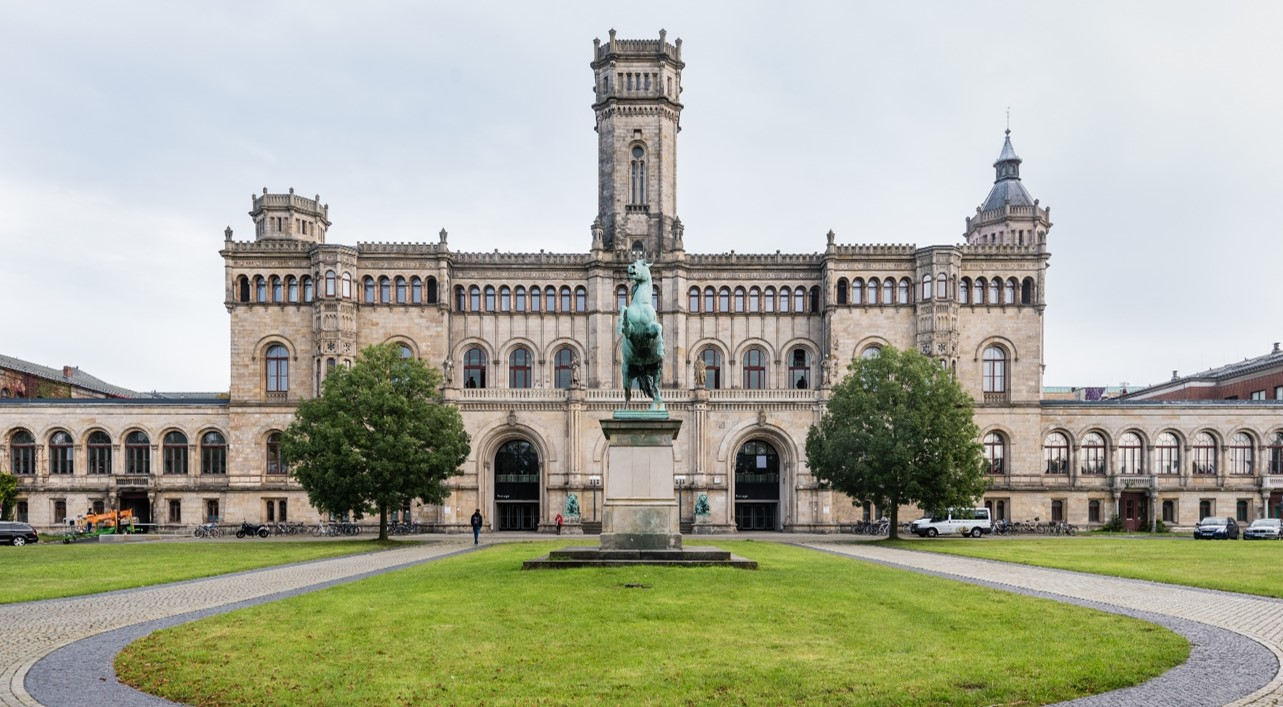
\includegraphics[width=0.65\textwidth]{figures/luh_default_presentation_title_image.jpg}}

% Title page: luhstyle
% \setbeamertemplate{title page}[luhstyle]
% % Add optional title image here
% \addtitlepageimage{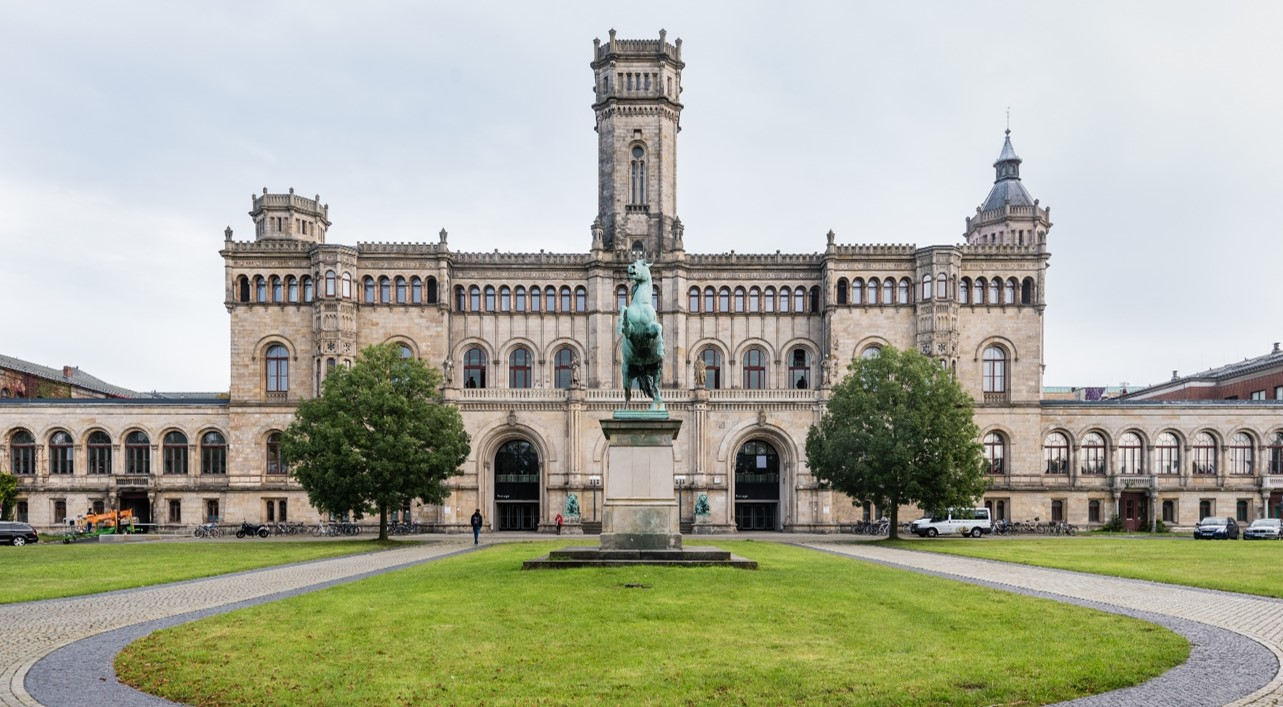
\includegraphics[width=0.75\textwidth]{figures/luh_default_presentation_title_image.jpg}}

\author[Abedjan \& Lindauer]{Ziawasch Abedjan \& Marius Lindauer\\[1em]
	
\includegraphics[height=\logoheight]{../latex_main/figures/luh_logo_rgb_0_80_155.pdf}\qquad
	
\includegraphics[height=\logoheight]{../latex_main/figures/DBIS_Kurzlogo.png}\qquad

\includegraphics[height=\logoheight]{../latex_main/figures/TNT_darkv4}\qquad

\includegraphics[height=\logoheight]{../latex_main/figures/L3S.jpg}	}
\date{Summer Term 2022; \hspace{0.5em} {
\includegraphics[height=1.5em]{../latex_main/figures/Cc-by-nc-sa_icon.svg.png}}; based on \href{https://ds100.org/fa21/}{[DS100]}
}


%%% Custom Packages
%----------------------------------------------------------------------
% Create dummy content
\usepackage{blindtext}

% Adds a frame with the current page layout. Just call \layout inside of a frame.
\usepackage{layout}


%%% Macros
%\renewcommand{\vec}[1]{\mathbf{#1}}
% \usepackage{bm}
%\let\vecb\bm

\title[Regression]{DS: Ordinary Least Squares}
\subtitle{Unique Solution?}

\graphicspath{ {./figure_ols/} }
%\institute{}


\begin{document}
	
	\maketitle
	\begin{frame}{Does a solution always exist?}
	    \begin{itemize}
	        \item For all models so far, our goal has been to determine the value of $\vect{\vect{\theta}}$ that minimizes some average loss.
	        \item The minimum value of both mean squared error and mean absolute error is 0.
	    \end{itemize}
	    \begin{equation*}
	        MSE(\vect{y},\hat{\vect{y}}) = \frac{1}{n}\sum\limits_{i=1}^n(y_i \hat{y_i})^2 \hspace{1cm} MAE(\vect{y},\hat{\vect{y}}) = \frac{1}{n}\sum\limits_{i=1}^n|y_i \hat{y_i}|
	    \end{equation*}
	    
	    \begin{itemize}
	        \item This means, there is always at least one model parameter that minimizes average loss.
	    \end{itemize}
	\end{frame}
	
	
	
	\begin{frame}{Does a solution always exist?}
	
	    \vspace{-2em}
	    \begin{columns}
	    
	        \begin{column}{.6\textwidth}
	        
	                \begin{itemize}
	                    \item Constant model with squared loss: 
	                    \begin{itemize}
	                        \item Any set of values has a unique mean.
	                        \item Thus, in this case, a unique solution always exists.
	                    \end{itemize}
	                    \item Simple linear model with squared loss: 
                        \begin{itemize}
                            \item Any set of non-constant values has a unique mean, SD, and correlation coefficient.
                        \end{itemize}
                        \item Constant model with absolute loss:
                        \begin{itemize}
                            \item This is unique when there is an odd number of y values.
                            \item But when there is an even number of y values, there are infinitely many solutions!
                            \begin{itemize}
                                \item In such a case, any value of $\vect{\theta}$ between the “middle two” values minimized MAE
                            \end{itemize}
                        \end{itemize}
                        
	                \end{itemize}
	                
	        \end{column}
	        
	        
	        
	        \begin{column}{.4\textwidth}
	        
	            \bigksip
	                \begin{equation*}
	                    \hat{\vect{\theta}} = mean(y)
	                \end{equation*}
	                
	                \begin{equation*}
	                    \hat{{\theta}_1} = r\frac{\sigma_y}{\sigma_x} \hspace{1cm}
	                    \hat{{\theta}_0} = \bar{y} - \hat{{\theta}_0}\bar{x}
	                \end{equation*}
	                
	                
	                \begin{equation*}
	                    \hat{\vect{\theta}} = median(y)
	                \end{equation*}
	                
	        \end{column}
	    \end{columns}
	\end{frame}
	
	
	
	\begin{frame}{Understanding the solution matrices}
	    Typically, $n$ is much larger than $p$.
	    \begin{figure}
	        \centering
	        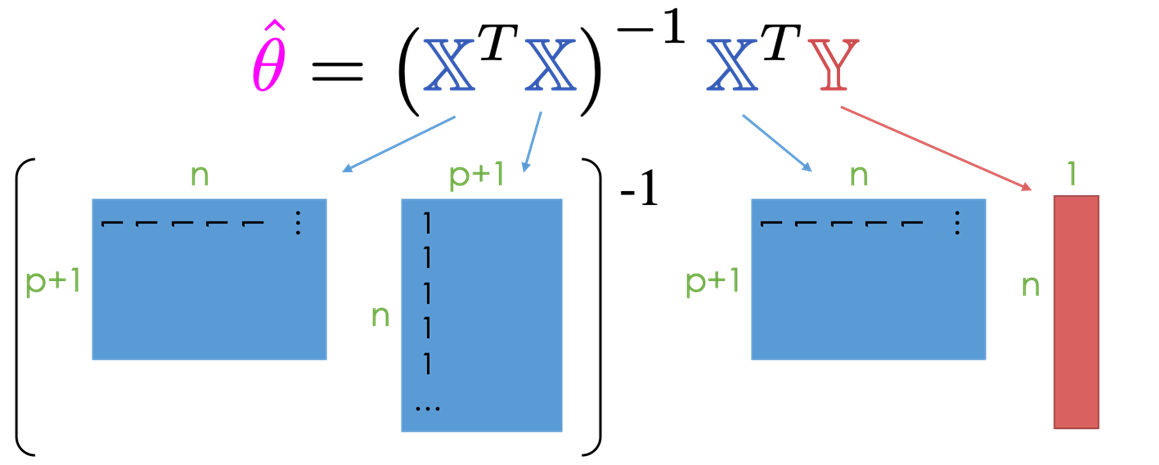
\includegraphics[scale=.45]{Bild13}
	    \end{figure}
	\end{frame}
	
	
	\begin{frame}{Understanding the solution matrices}
	Typically, $n$ is much larger than $p$.
	    \begin{figure}
	        \centering
	        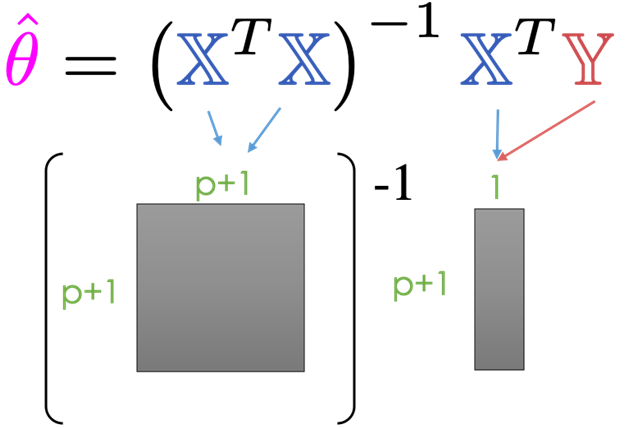
\includegraphics[scale=.45]{Bild14}
	    \end{figure}
	\end{frame}
	
	\begin{frame}{Understanding the solution matrices}
	    The Normal Equation:

	    \begin{figure}
	        \centering
	        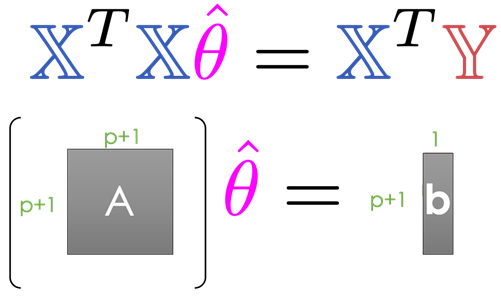
\includegraphics[scale=.45]{Bild15}
	    \end{figure}
	    Our optimal parameter vector can be thought of as the solution to a set of $p + 1$ equations, with $p + 1$ unknowns. 

	\end{frame}
	
	
	\begin{frame}{Does a unique solution always exist?}
	   Let’s consider our optimal $\vect{\theta}$ for the multiple linear regression model:
	   \begin{equation*}
	       \hat{\vect{\theta}} = (\vect{X}^\intercal\vect{X})^{-1} \vect{X}^\intercal\vect{Y}
	   \end{equation*}
	    
	    \begin{itemize}
	        \item As mentioned previously, at least one solution always exists.
	        \begin{itemize}
	            \item Intuitively, we can always draw a line of best fit for a given set of data. There may be multiple lines that are “equally good”.
	        \end{itemize}
	        \item When does a unique solution for   $\hat{\vect{\theta}}$  exist?
            \begin{itemize}
                \item When     $\vect{X}^\intercal\vect{X}$      is invertible. If it is not invertible, a unique solution does not exist.
                \item In such a case, there will be infinitely many values of theta that minimize average squared loss.
                \item If there are infinitely many “optimal” choices of coefficients, it’s unclear which to use.
                \item We want a unique solution.
            \end{itemize}
	    \end{itemize}

	\end{frame}
	
	
	\begin{frame}{Invertibility of  $\vect{X}^\intercal\vect{X}$ }
	    When is $\vect{X}^\intercal\vect{X}$ invertible?
	    \begin{itemize}
	        \item $\vect{X}^\intercal\vect{X}$ is invertible if and only if it is full rank.
	        \begin{itemize}
	            \item The shape of    $\vect{X}^\intercal\vect{X}$ is $(p + 1) \times (p + 1)$. Invertibility is only defined for square matrices.
	            \item The rank of a matrix is the number of linearly independent columns (or rows) it contains.
	            \item This is one of several conditions of the “invertible matrix theorem.”
	        \end{itemize}
	        \item   $\vect{X}^\intercal\vect{X}$ and $\vect{X}$ have the same rank.
	        \begin{itemize}
	            \item The proof is beyond the scope of this class.
	        \end{itemize}
	        \item The maximum possible rank of   $\vect{X}^\intercal\vect{X}$  is $p + 1$.
	        \item Thus, $\vect{X}^\intercal\vect{X}$   is invertible if and only if $\vect{X}$ has rank $p + 1$ (full column rank). 
            \begin{itemize}
                \item That is, a unique solution for the least squares estimate exists if and only if all columns of $\vect{X}$ are linearly independent.
                \item \alert{Trick}: Try to add a very small $\epsilon$ to the diagonal if it is not invertible
            \end{itemize}
	    \end{itemize}
	\end{frame}
	
	
	\begin{frame}{Invertibility of  $\vect{X}^\intercal\vect{X}$ }
	    When does our design matrix    $\vect{X}$   not have full column rank?
	    \begin{itemize}
	        \item When some features in our design matrix are linear combinations of other features.
	        \begin{itemize}
	            \item If “Width”, “Height”, and “Perimeter” are all columns, $\vect{X}$ will not have full rank, since\\ Perimeter = 2 $\cdot$ Width + 2 $\cdot$ Height (linear combination).
	            \item When we discuss one-hot encoding, this is something to be aware of.
	        \end{itemize}
	        \item  When our design matrix has more columns than rows (i.e. it is “fat”).
	        \begin{itemize}
	            \item In the normal setting, n > p + 1 (we typically have more observations than features). 
	        \end{itemize}
	    \end{itemize}
	    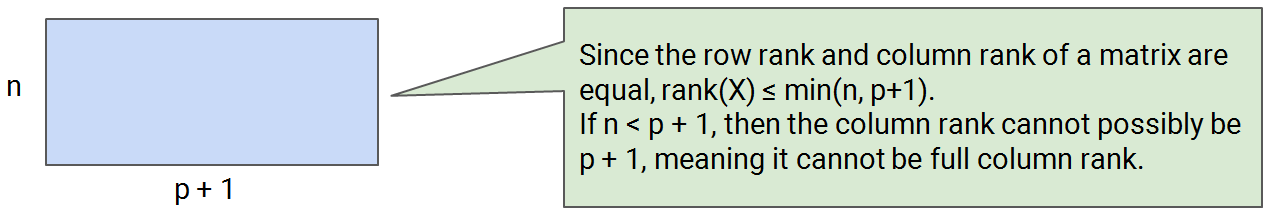
\includegraphics[scale=.45]{Bild16}
	\end{frame}
\end{document}